\documentclass{bredelebeamer}




%%%%%%%%%%%%%%%%%%%%%%%%%%%%%%%%%%%%%%%%%%%%%%%%



\title[Conception logicielle]{Conception logicielle}
% Titre du diaporama

\subtitle{Soutenance de stage}
% Sous-titre optionnel

\author{Nathan Michanol - Master 1 MIAGE\\}

% La commande \inst{...} Permet d'afficher l' affiliation de l'intervenant.
% Si il y a plusieurs intervenants: Marcel Dupont\inst{1}, Roger Durand\inst{2}
% Il suffit alors d'ajouter un autre institut sur le modèle ci-dessous.

\institute[ ]
{
  
\includegraphics[scale=0.3]{images/logoNanterre.jpg}\\
  
  Référent : Prof. Marie-Pierre Gervais\\
  Tuteur : M. Raphaël Martin
}


\date{3 juillet 2018}
% Optionnel. La date, généralement celle du jour de la conférence

\subject{Conception logicielle}
% C'est utilisé dans les métadonnes du PDF



\logo{

\includegraphics[scale=0.5]{images/logo_psa.png}
}


%%%%%%%%%%%%%%%%%%%%%%%%%%%%%%%%%%%%%%%%%%%%%%%%%%%%%%%%%%%%%%%%%%%%%
\begin{document}

\begin{frame}
  \titlepage
	
\end{frame}


\begin{frame}{Sommaire}
  \tableofcontents
  % possibilité d'ajouter l'option [pausesections]
\end{frame}




\section{L'entreprise Groupe PSA}

%\subsection{Secteurs d'activité de l'entreprise}
\begin{frame}{Secteurs d'activité de l'entreprise}
	\begin{itemize}
		\item Constructeur automobile français
		\bigskip
		\item Présence industrielle et commerciale internationale
		\bigskip
		\item 4 sites de recherche et développement en France
	\end{itemize}
\end{frame}

\begin{frame}{Le service SEPH}
	\begin{enumerate}
		\item «Software Engineering Powertrain and Hybrid»
		\bigskip
		\item Mission :
		\bigskip
		\begin{itemize}
			\item Développement de la partie applicative des logiciels pour le contrôle moteur et la supervision machine électrique
			\bigskip
		\end{itemize}
	\item Activités :
	\bigskip
		\begin{itemize}
			\item Equipes Productions des logiciels embarqués
			\bigskip
			\item Equipe Outils : maintenance et évolution de la chaîne outillée
			\bigskip
			\item Maîtrise d’oeuvre et maîtrise d'ouvrage
			\bigskip
			\item Méthode de travail : Model Based Design
		\end{itemize}
	\end{enumerate}
\end{frame}

\begin{frame}{Le cycle en W}
	\begin{figure}
		\centering
		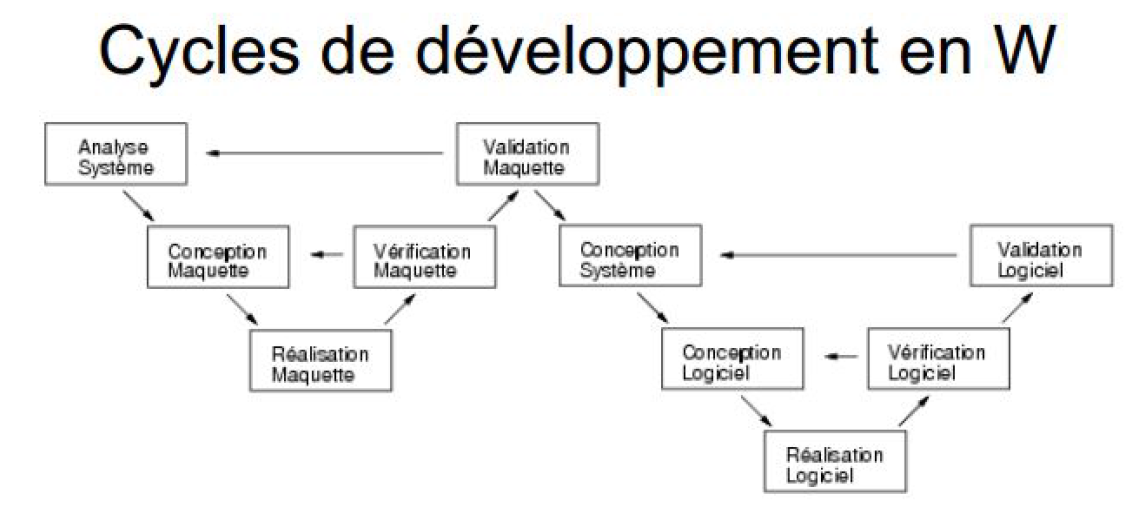
\includegraphics[scale=0.35]{images/cycleW.png}
	\end{figure}
\end{frame}

\section{La mission}

\begin{frame}{Contexte}
	\begin{figure}
		\centering
		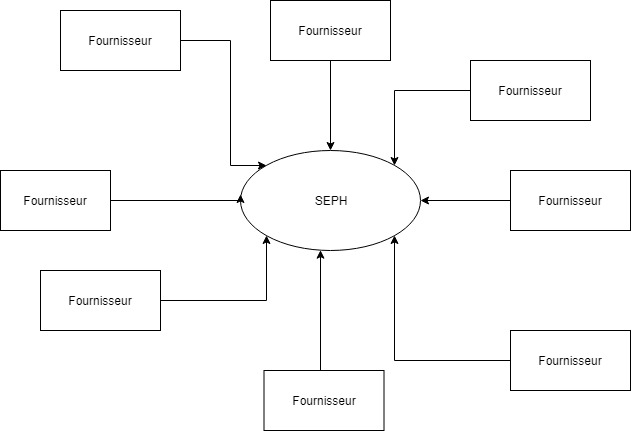
\includegraphics[scale=0.35]{images/schemasEntrant.jpg}
	\end{figure}
\end{frame}

\begin{frame}{Les livrables}
	\begin{figure}
		\centering
		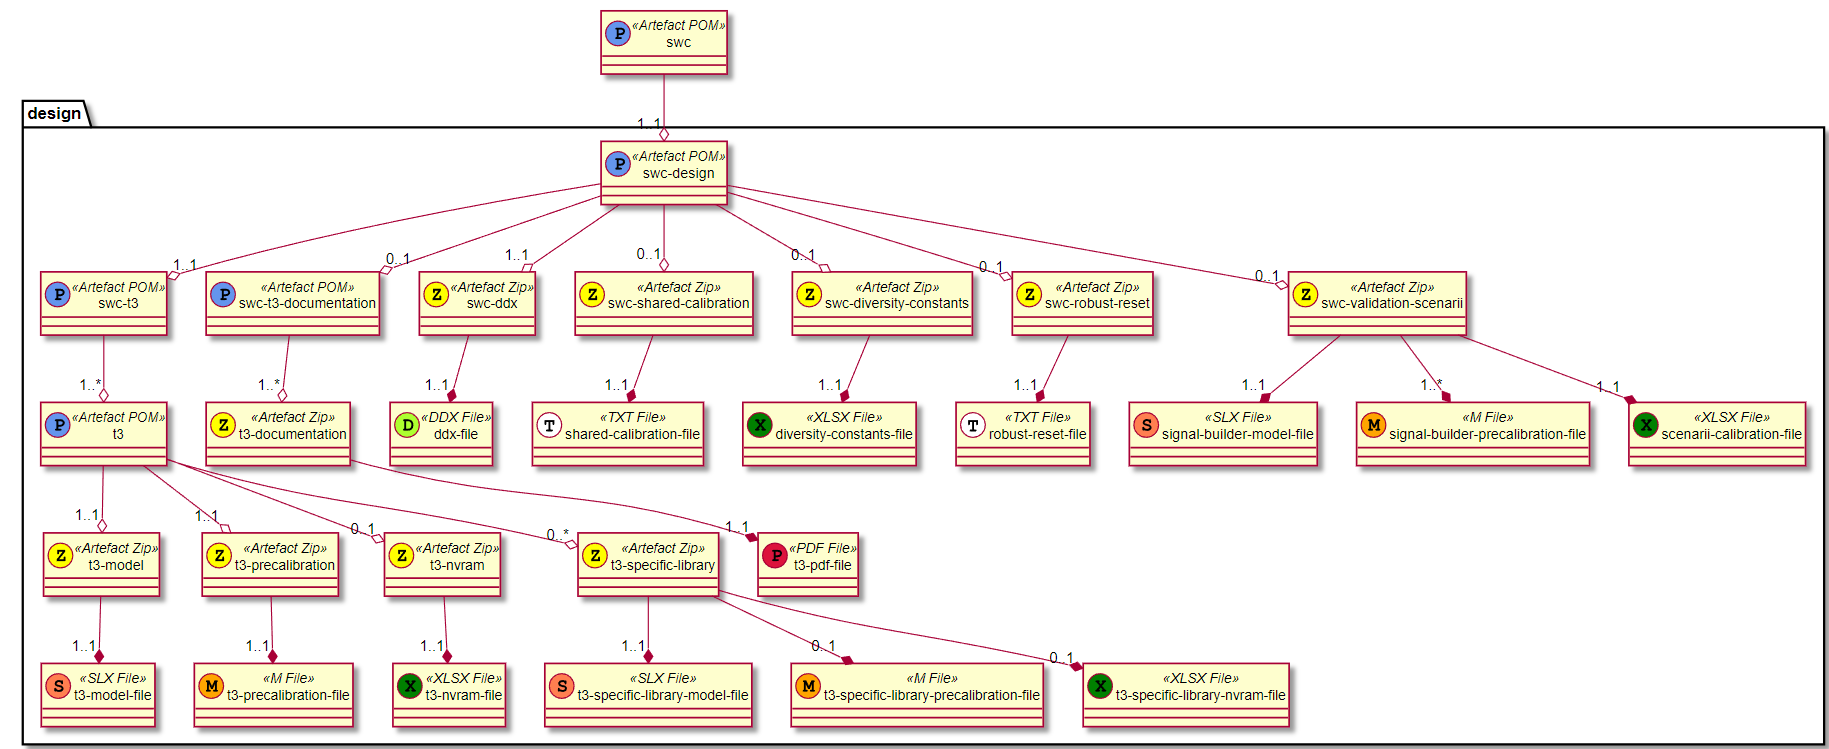
\includegraphics[scale=0.3]{images/livrables.png}
	\end{figure}
\end{frame}

\begin{frame}{Architecture de la future plateforme de livraison}
	\begin{figure}
		\centering
		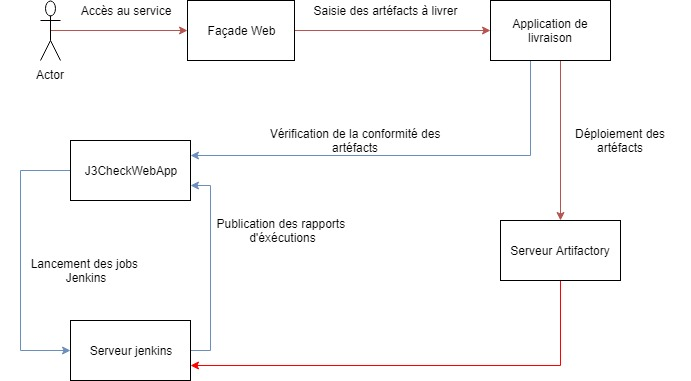
\includegraphics[scale=0.35]{images/workflow.jpg}
	\end{figure}
\end{frame}

\begin{frame}{Les technologies}
	\begin{figure}
		\centering
		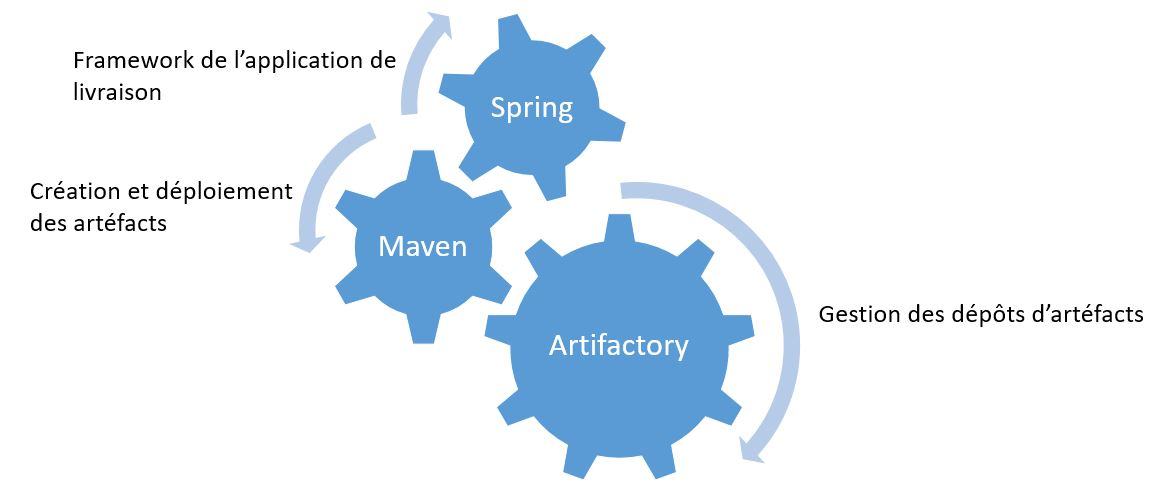
\includegraphics[scale=0.45]{images/techno.jpg}
	\end{figure}
\end{frame}

\begin{frame}{Méthodologie}
	\logo{
		
\includegraphics[scale=0.5]{images/scrumLogo.png}
	}
	\begin{itemize}
		\item Méthode agile Scrum
		\bigskip
		\item Sprint de 3 semaines organisé lors du Sprint planning
		\bigskip
		\item 1 Product Owner
		\item 1 Scrum Master
		\bigskip
		\item Daily Meeting
		\item Backlog Grooming
	\end{itemize}
\end{frame}

\begin{frame}{Exemple de Story}
	\begin{figure}
		\centering
		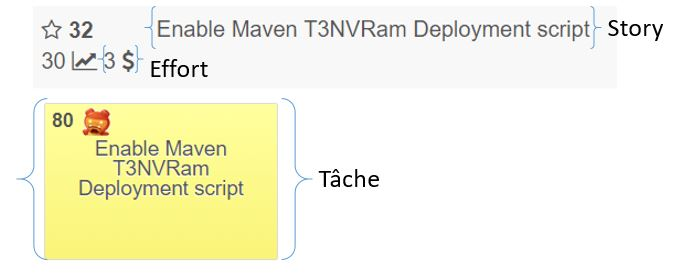
\includegraphics[scale=0.65]{images/storySample.jpg}
	\end{figure}
\end{frame}



\begin{frame}{Travail effectué}
	\begin{figure}
		\centering
		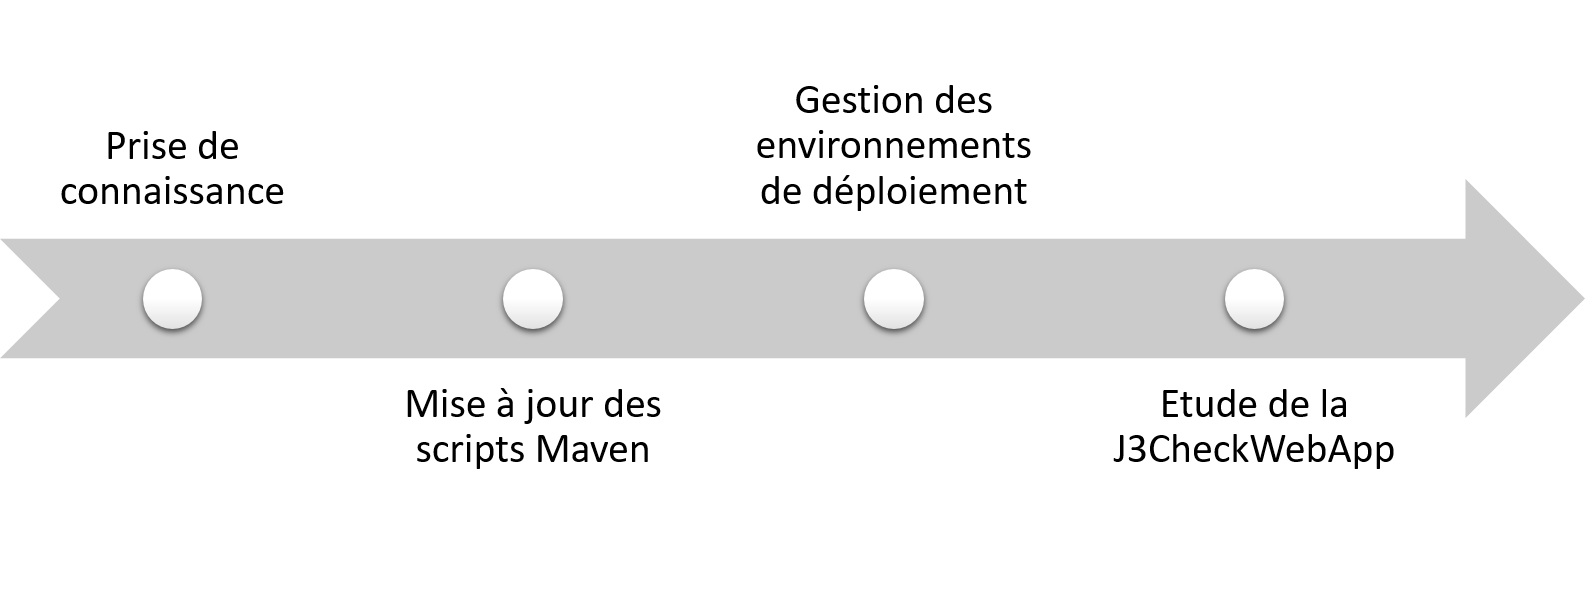
\includegraphics[scale=0.4]{images/chronoWork.png}
	\end{figure}
\end{frame}


\section{Conclusion}
\begin{frame}{Conclusion}
	Bilan des connaissances :
	\begin{itemize}
		\bigskip
		\item Première expérience agile profesionnelle
		\bigskip
		\item Apprentissage de nouveaux outils (Maven, Artifactory)
		\bigskip
		\item Premier contact avec le métier d'ingénieur
	\end{itemize}
		\bigskip
		Bilan personnel :
	\begin{itemize}
		\bigskip
		\item Immersion dans une grande entreprise
		\bigskip
		\item Orientation vers la maitrise d'oeuvre
	\end{itemize}
\end{frame}

\section{Annexes}
\begin{frame}{Annexes}
	\begin{figure}
		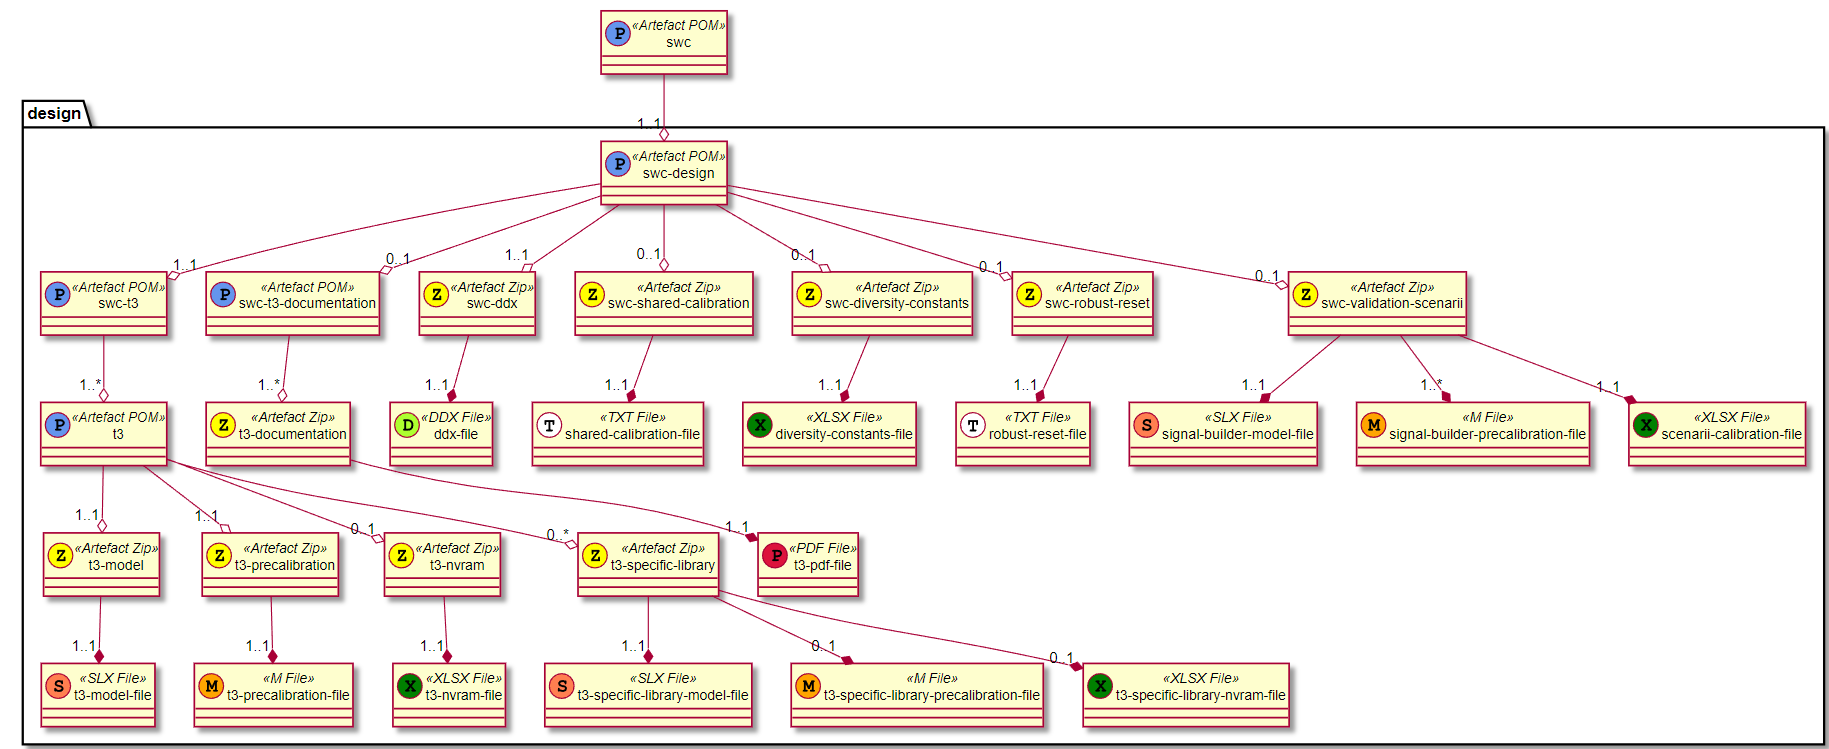
\includegraphics[scale=0.3]{images/livrables.png}
	\end{figure}
\end{frame}
\end{document}
